\documentclass{article}

\usepackage{subfig}
\usepackage{float}
\usepackage{graphicx}
\usepackage{algorithm}
\usepackage{algpseudocode}
\usepackage{changepage}
\usepackage{amsmath}
\usepackage[driver=pdftex]{geometry}




\begin{document}
\begin{titlepage}
	
	
	\begin{center}
		\vspace{2 cm}
		{\Large \textsc{Simone Quadrelli} }
	\end{center}
	
	
	\begin{figure}[H]
		\vspace{2 cm}
		\centering
		
\includegraphics[width=0.30\linewidth]{tesiSCIENZE_TECNOLOGIE.jpg}
		
	\end{figure}
	
	\begin{center}
		\vspace{2 cm}
		{\Large \textsc{Fruit classification} }
	\end{center}

	\par
	\vspace{3 cm}
	
	\begin{center}
		{\large Academic year 2018 - 2019}
	\end{center}
\end{titlepage}

\pagenumbering{gobble}
\newpage 
\pagenumbering{roman}
\tableofcontents
\listoftables
\listoffigures
\newpage

\pagenumbering{arabic}

\section*{Abstract}
An abstract summarizes, usually in one paragraph of 300 words or less, the major aspects of the entire paper in a prescribed sequence that includes: 1) the overall purpose of the study and the research problem(s) you investigated; 2) the basic design of the study; 3) major findings or trends found as a result of your analysis; and, 4) a brief summary of your interpretations and conclusions.
\\\\\\
The aim of the project is to investigate the ability of KNN, SVM and CNN to classify images of fruits and vegetable. The feature vectors are made of rgb and grayscale. First the features were extracted, then a feature reduction is performed. KNN and SVM performance are computed with different parameters and number of features. In the end, CNN are applied to the whole features. CNN perform the best, but KNN reaches a surprisingly high accuracy. Overall, CNN are the best model to choose. Grayscale features are usefull however rgb features are more meaningful. Despite its semplicity, KNN have remarkable performance.
\section{Introduction}
The objective of this project is to classify a variety of fruits and vegetables whose images are stored in a recently released dataset.\\
Fruit and vegetable classification is a challenging task, there are two different kind of problems that must be overcome: vegetables and fruits within the same class can differ in shape and colour due to maturity and growth. On the countrary, vegetables and fruits in different classes, such as red apples or grapes, may be very similar both in textures and in colours. 
Fruit and vegetables classification has a key role in many industries: it can be exploited to make agriculture more autonomous than ever before in history, but it can also be applied to all stages of the supply chain to assess the quality of the products from the producer to the consumer. 
The ability of harvesting robots can be enhanced by enforcing fruit and vegetables recognition, indeed it may allow them to recognize not only the type of fruit or vegetable but also its maturity or whether it is rotten. Moreover, autonomous classification provides more consistent quality assessment since it does not depend of the opinion of different workers.
\\
The projects will analyze the classification performance of three machine learning algorithms on different fruits. The k-nearest neighbour (KNN) algorithm was used to compute a baseline, a more sophisticated one, the support vector machines (SVM) algorithm was later used for classification. The last approach was to construct a convolutional neural network (CNN) because they are known to suit well image classification problems. The are two different kind of features that were extracted to feed the algorithms: the grayscale and the rgb representation of the images.\\
The objective of the project are:
\begin{enumerate}
\item Analyze the accuracy result achieved with grayscale features
\item Study the improvement in performance induced by rgb features
\item Compare the performance of KNN with that of more sophisticated algorithms
\end{enumerate}

\section{Dataset and Features}
The analyzed dataset, known as \textit{Fruits 360}, was originally published in 2017  by Horea Muresan and Mihai Oltean to address fruit and vegetable classification \cite{dataset}. The existence of either too small datasets or too low-quality dataset was the most compelling problem.  On the countrary, this dataset provides more that 70000 images of 114 different fruits and vegetables. Each image has a definition of 100 $\times$ 100 pixels. To increase the reliability of the results, it contains images of rotated fruits and vegetables. However those images make the training process much harder .
As the authors explain, the dataset was produced as follows: fruits and vegetables were planted in the shaft of a low speed motor (3 rpm) and a short movie of 20 seconds was recorded. However, due to the variations in the lighting conditions, the background was not uniform and a dedicated algorithm was exploited to extract the fruit from the background. The images were of such high quality that no preprocessing was required.
It is also worth noticing that the dataset was already splitted in train and test set, therefore no further splitting was required.\\
Fruits and vegetables have several distinct visual characteristics that can be extracted from the images. Colour, shape, size and texture are the most commonly used features\footnote{Features are the characteristics of an object that can distinguish it from other objects} in image classification.  Among all the possible feauters that can be extracted from an image, colours features play a key role in fruit and vegetable classification. Indeed, they seem to be suitable for the problem and their computation is very fast and efficient \cite{review}. The project focuses on the grayscale and rgb representation of the images. \\
The following lines introduce the reader to some concept of colour spaces and colour representation.
Colour spaces are a specific organization of colors the allows to  reproduce the representation of colours. Two different colour spaces were exploited in this project: grayscale and the rgb.
\subsection{RGB colour space}
The RGB colour model is an additive colour model, meaning that red, green and blue are added together to reproduce an wide array of colors. A color in the RGB colour model is described by indicating how much of the red, green, and blue is included. The colour of a pixel is expressed as an RGB triplet (R,G,B). Each component can vary from 0 to 255, since each channel is represented by a byte.


\subsection{Grayscale colour space}
Since the dataset contains rgb images, it was necessary to extraxt a grayscale representation of the pixels to be used as features.
In grayscale representation each pixel is a byte, meaning that the possible values it can be in range from 0 to 255. \\
The conversion algorithm implemented by the library \textit{imager} is the Luma algorithm. Each rgb channel $R, G, B$ of a pixel are passed to a function $\Gamma(x)$ to obtain its transformation, respectively $R', G', B'$. \\
The $\Gamma$ function is defined as: 
\begin{equation}
 x' = \Gamma(x) = Ax^{\gamma}
\end{equation}
where $x$ in the pixel intensity, $A$ is a scalar whose value is often $1$ and $\gamma$ is usually $\frac{1}{2.2}$.\\
To obtain the final grayscale representation  $y$ of a pixel $x$, the following linear transformation is applied: \cite{grayscaleconversion}
\begin{equation}
 y = 0.21 R' + 0.71 G' + 0.07  B'
\end{equation}


\section{Data analysis}
This section provides the reader an insight of the procedure used to analyze the data, it also provides a commantary of the results.\\
The procedure described in the section is the same for both the grayscale features and the rgb features, however the differ in the topology of the convolutional neural network. Algorithm \ref{schema} provides a brief overview of the analysis.

\begin{algorithm}[H] 
   \caption{Schema of the analysis} \label{schema}
    \begin{algorithmic}[1]
    \State Feature extraction
    \State Dimensionality reduction
    \State Extraction of the most significant features
    \State Construction of a baseline using knns
    \State Evaluation of svm
    \State CNN
\end{algorithmic}
\end{algorithm}

\subsection{Feature extraction and dimensionality reduction}
The first major step in the analysis is the data extraction and the computation of the data matrix and the vector of the labels concerning the following fruits: \textit{Apple Golden 1}, \textit{Apple Golden 2}, \textit{Apple Red 2}, \textit{Apple Red 1}, \textit{Banana}, \textit{Apricot}, \textit{Blueberry}. \\
As previously stated, the dataset contains 100x100 pixels images, therefore the data matrix with rgb features has 409440000 elements. Bearing that in mind, the images are rescaled to 50 $\times$ 50 pixels to reduce the computational complexity of the problem. 
The feature vector of each image is extracted by the functions of the library \textit{imager}. Once all the data vectors are extracted, a data matrix is created. Each row of the matrix contains the linearized representation of the image. At the same time a vector of labels is computed.\\
Most learning algorithms are exponentially slow in the number of the feature or at least significantly slow down as the number of feature increases. Furthermore, it is reasonable to belive that many of the pixels are useless since they are just part of the background. As a result, Principal component analysis (PCA) is exploited to reduce the dimensionality of the data and select the most promising features. PCA is one of the most common technique to reduce the dimensionality of the data since it is very efficient and many libraries implement it. PCA computes all the principal components that can be seen as the axis along which data differ the most. Before applying pca data points $x$ are standardized in the following way to ease the problem:
\begin{equation}
 \frac{x - \mu}{\sigma}
\end{equation}
\noindent where $\mu$ is the mean value and $\sigma$ is the standard deviation of the data. \\
When using the grayscale features the execution time required to compute the PCA is 5 minutes and 30 seconds. However, the execution time required to compute the PCA is about 57 minutes for grb features\footnote{All time measurement rely on a Intel Core i5-7200U dual core processor and 8 GB DDR4 RAM}.

\begin{figure}[H] 
  \begin{adjustwidth}{-4cm}{-4cm}
     \subfloat{%
       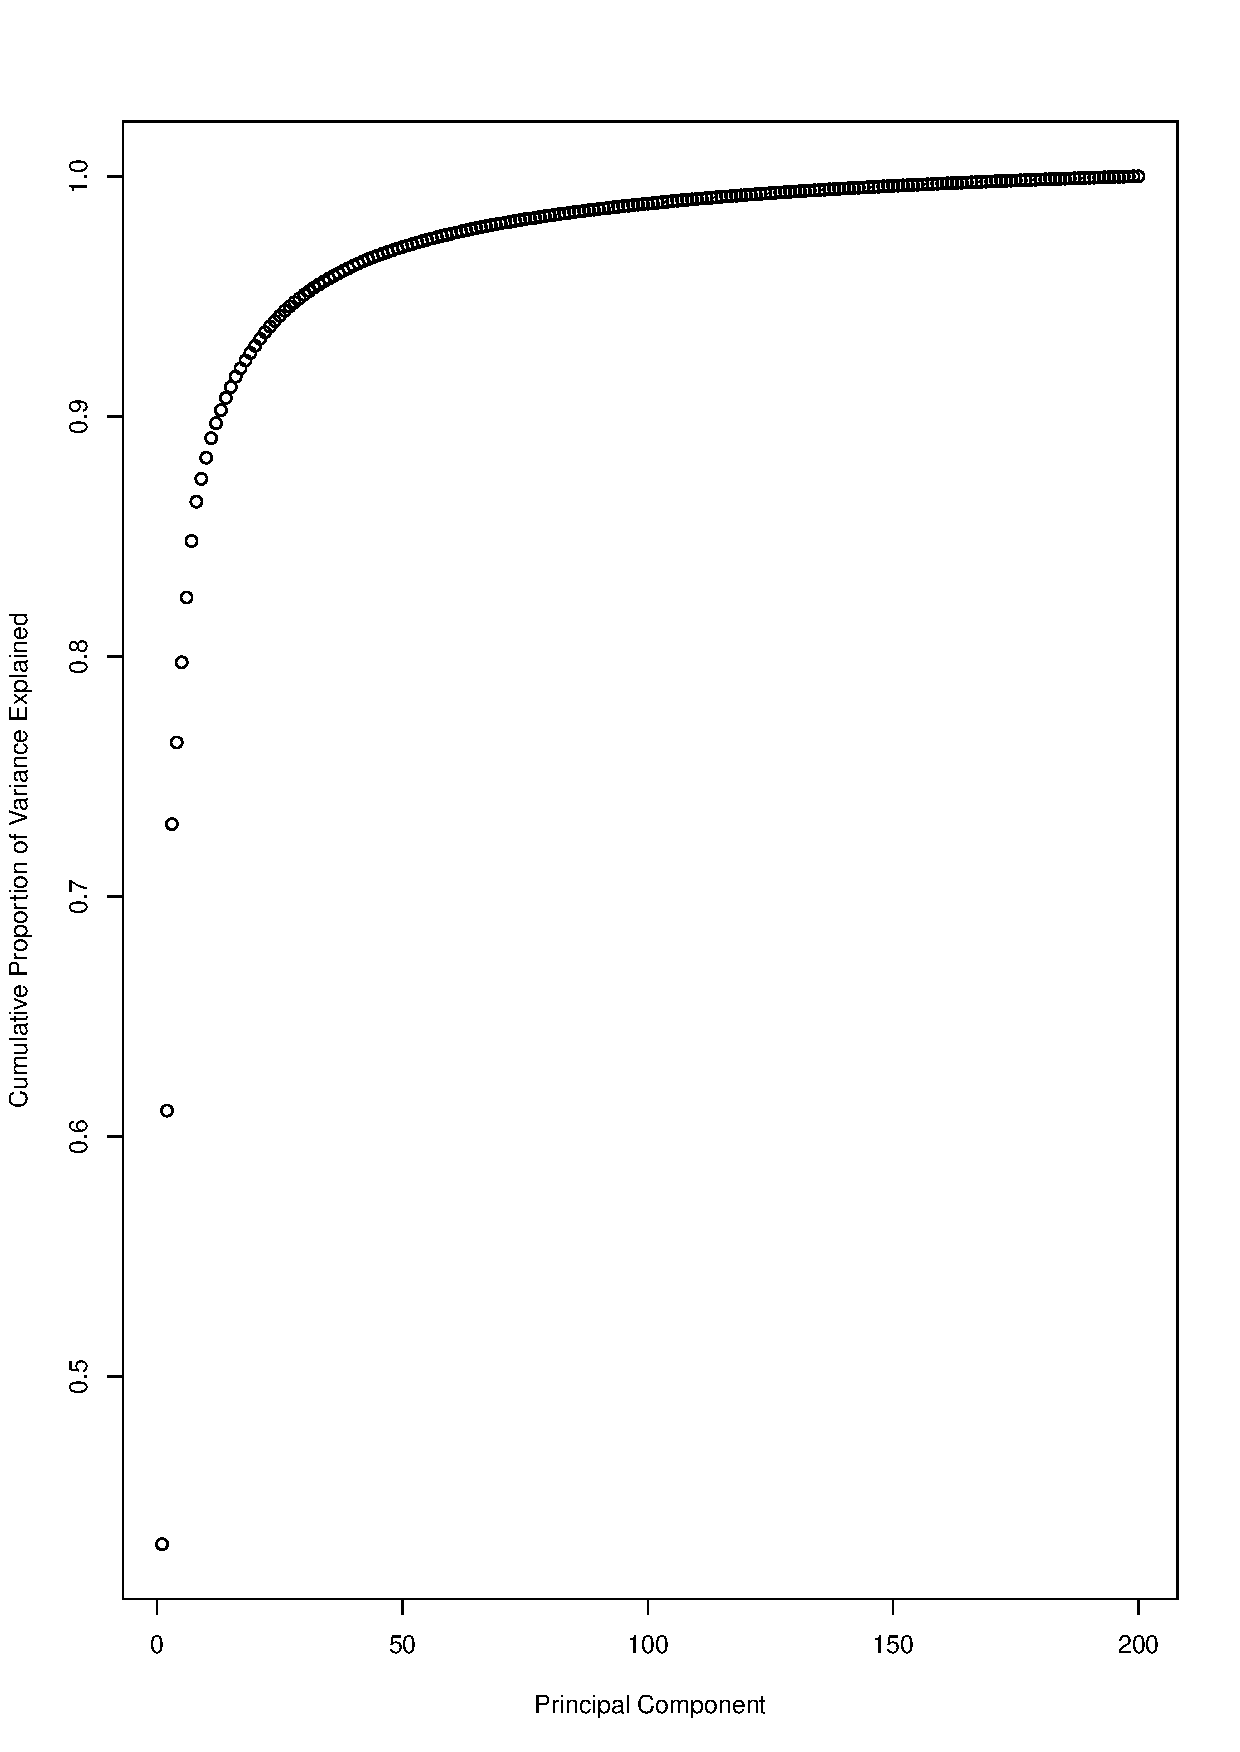
\includegraphics[scale=0.3]{../cumulative_variance_graysalce.pdf} 
     }
     \subfloat{%
    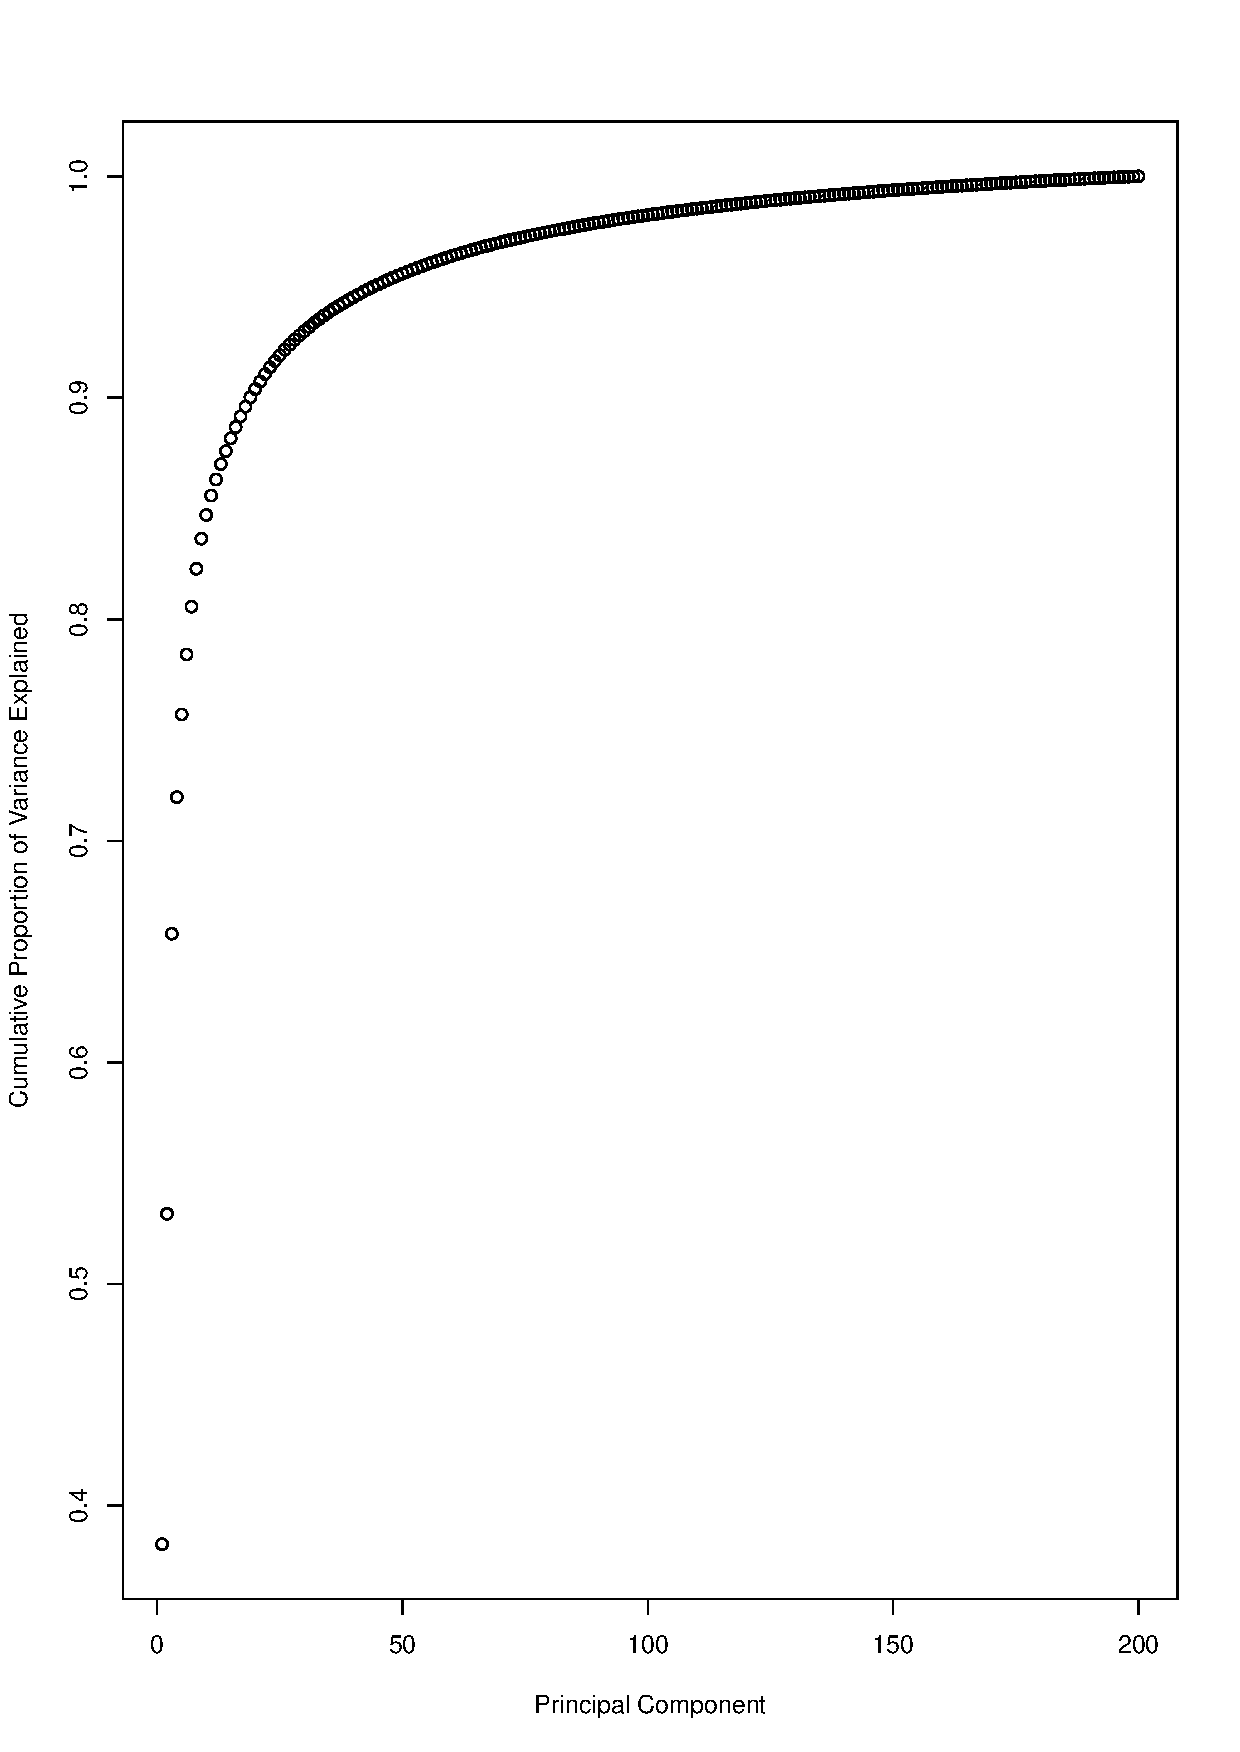
\includegraphics[scale=0.3]{../cumulative_variance_grb.pdf} 
     }
     \centering
     \caption{Cumulative variance explaind by the principal components}  \label{variance}
      \end{adjustwidth} 
   \end{figure}

\noindent As figure \ref{variance} show, in both cases, using 150 principal components is enough to explain all the variance in the data. However, having fixed the number of compunents, rgb components explain less variance than the grayscale components. To compare and analyze the performance of the learning algorithms the following set of principal components $\{3,10,50,100,150\}$ are used. The rationale behind this choice is to select the number of components that should give the best result having at the same time a fast execution time. \\
 
\subsection{Baseline and knn}
The k-nearest neighbours (knn) algorithm seems to be an appropriate choice to define a baseline because it is known to be one of the most efficient classification algorithm, even if it is very simple. Indeed, the knn classifies a test point with the labels of the closest training point. Moreover, in image classification it seems to perform quite as well as more sophisticated algorithms such as support vector machines. \cite{knnresults} \\
To evaluate the performace of the knn and the other algorithms, the most natural choice is the accuracy, defined as:
\begin{equation}
\text{accuracy}  = \frac{\text{Number of correct predictions}}{ \text{Total number of predictions}}
\end{equation}
\noindent The number of neighbours (k) chosen to construct the baseline are: $1,3,7,9,11$.
As can be seen from figure \ref{knnaccuracy}, there is no remarkable diffenrence in performace if the number of features exploited is 10 or more. On the other hand, when only three features are used the algorithm achieves lower performances. This difference is even more sharp when rgb features are involved\footnote{The figure on the left always refers to the result obtained using the grayscale features. The figure on the right refers to the result obtained using the rgb features.}, indeed the accuracy lies about 0.10 below the other accuracy lines.\\
The best number of features to select is 50, since with all the possible value of k knn performs best with 50 features.\\
If we limit our analysis, considering just the result of knn with at least 10 features 1-nn has the very best results, even if up to 7 neighbours there is no significant difference in performance.
Overall, knn reaches a very significant accuracy: the accuracy level  when considering rgb features reach up to 0.91, while the accuracy level reached using grayscale features is about 0.82. As expected the rgb features are more reliable and are associated with better results.\\
Overall, the best model is 1-nn with 50 features.

\begin{figure}[H] 
  \begin{adjustwidth}{-4cm}{-4cm}
     \subfloat{%
       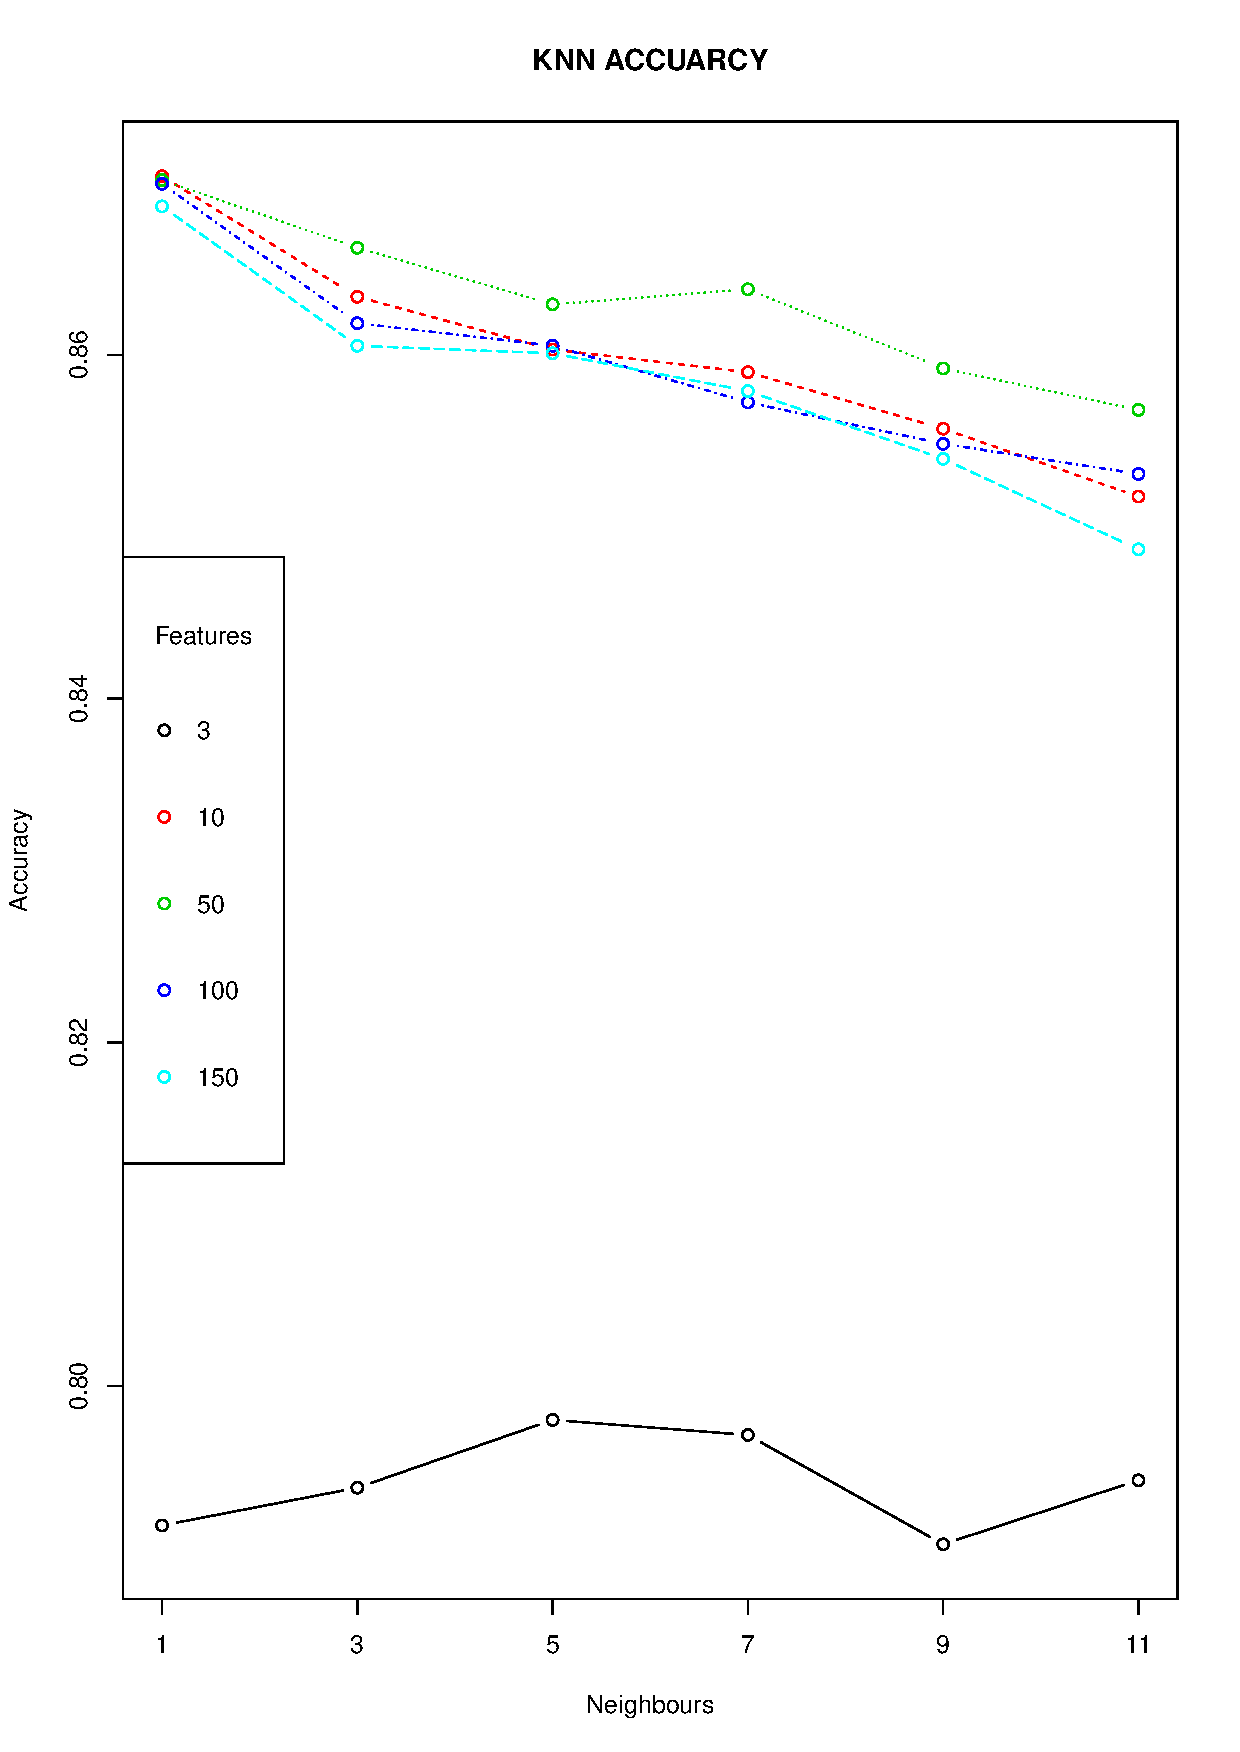
\includegraphics[scale=0.35]{../knn_accuracy_grayscale.pdf}
     }
     \subfloat{%
    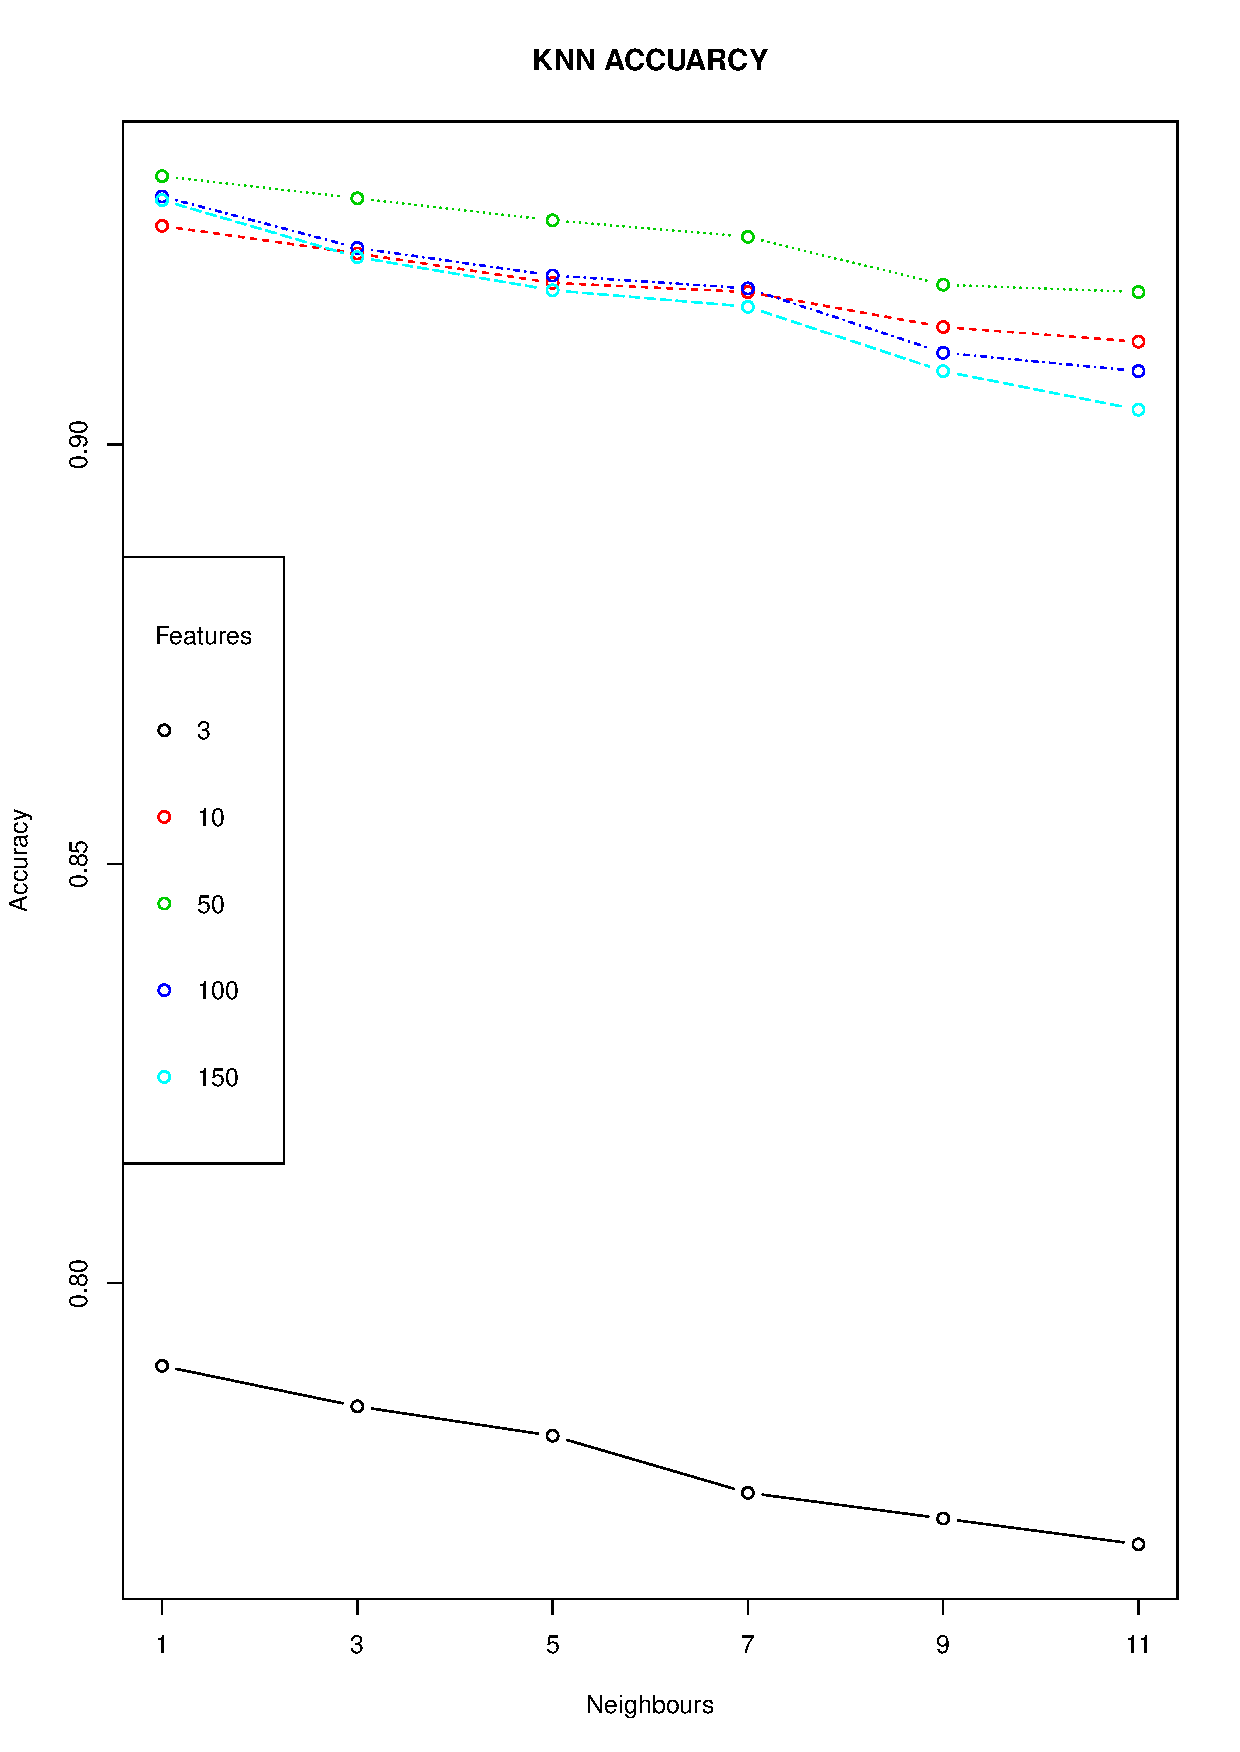
\includegraphics[scale=0.35]{../knn_accuracy_rgb.pdf}  
     }
     \centering
     \caption{Test accuracy knn}  \label{knnaccuracy}
      \end{adjustwidth}
   \end{figure}
   
\noindent The execution time of the algorithm is acceptable and does not exceed 30s. It is worth noticing that the execution time, given the number of features, have just neglegible variation when the number of neighbours changes.\\



   
\begin{figure}[H]  
  \begin{adjustwidth}{-4cm}{-4cm}
     \subfloat{%
       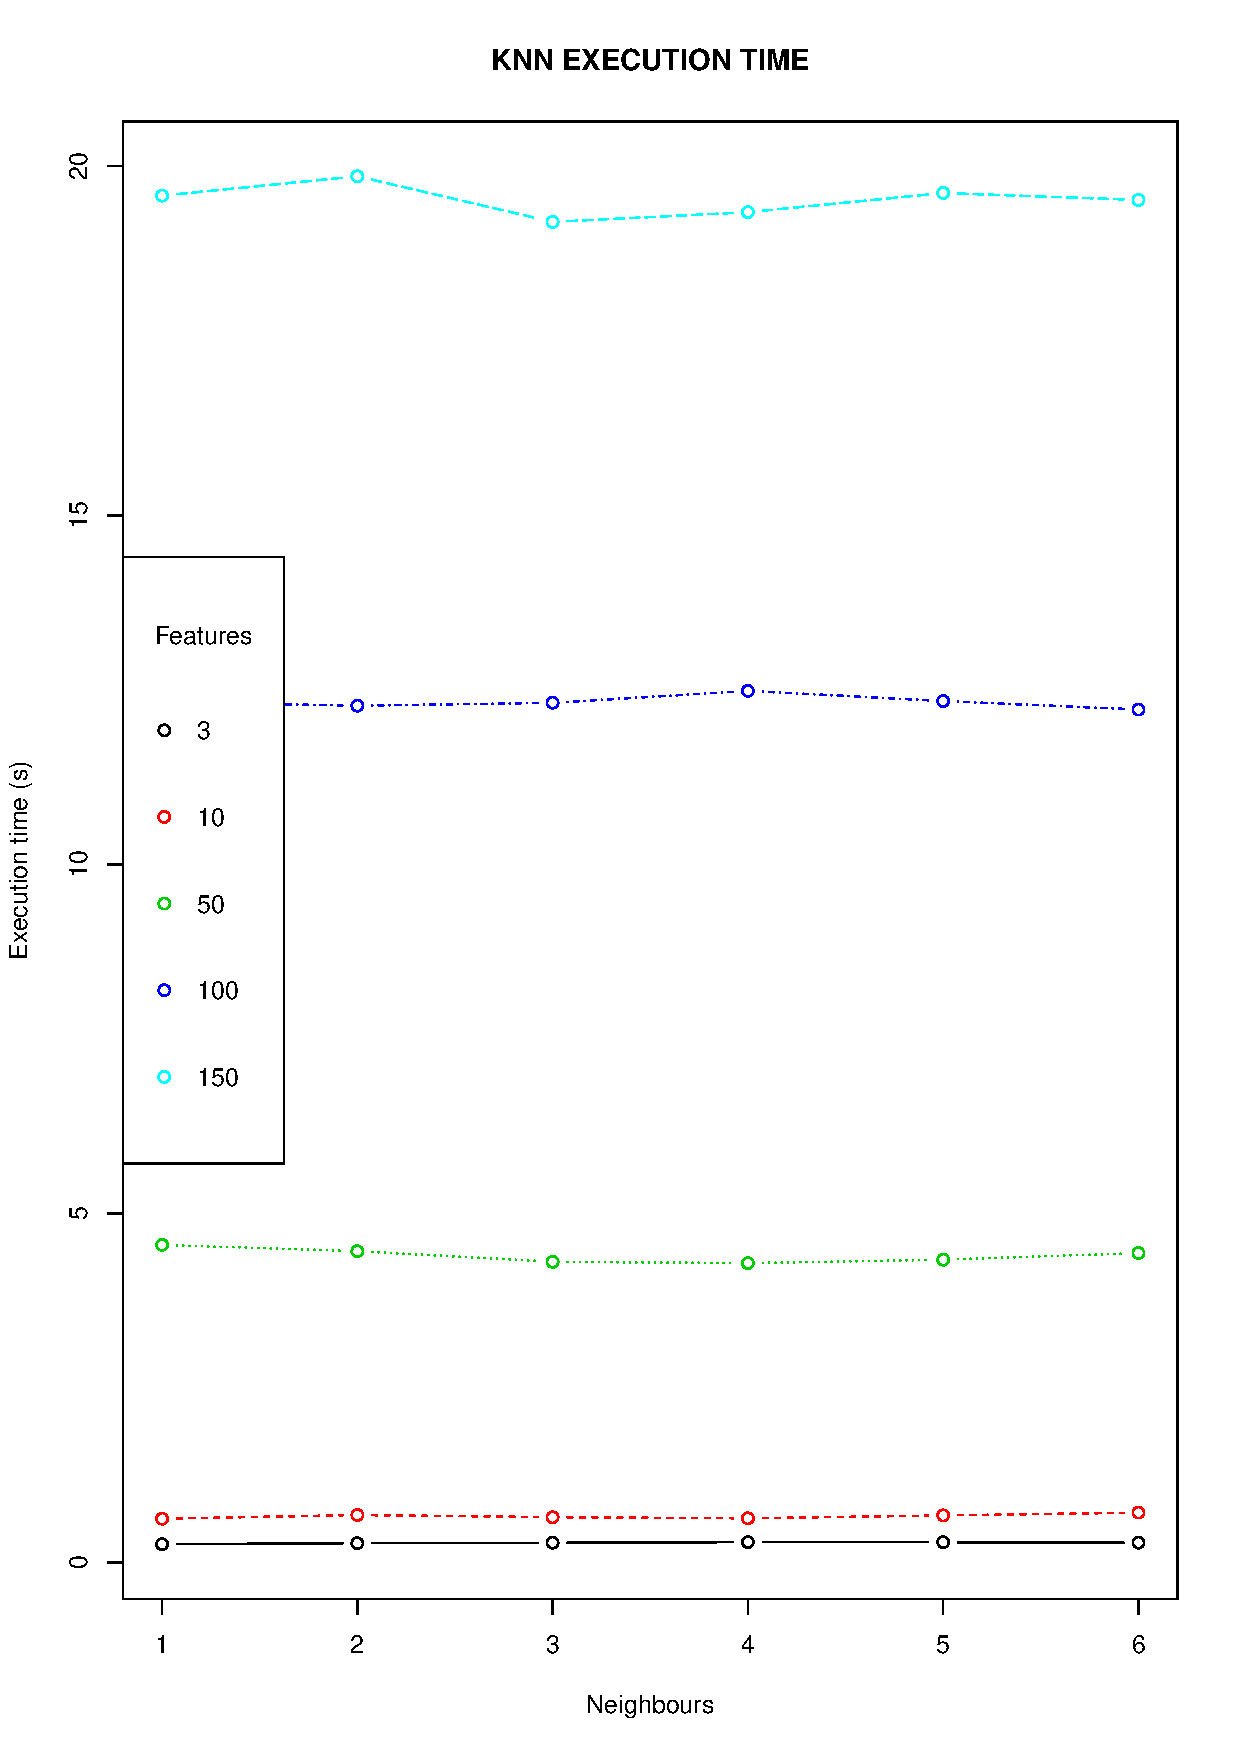
\includegraphics[scale=0.3]{../knn_time_grayscale.pdf}
     }
     \subfloat{%
    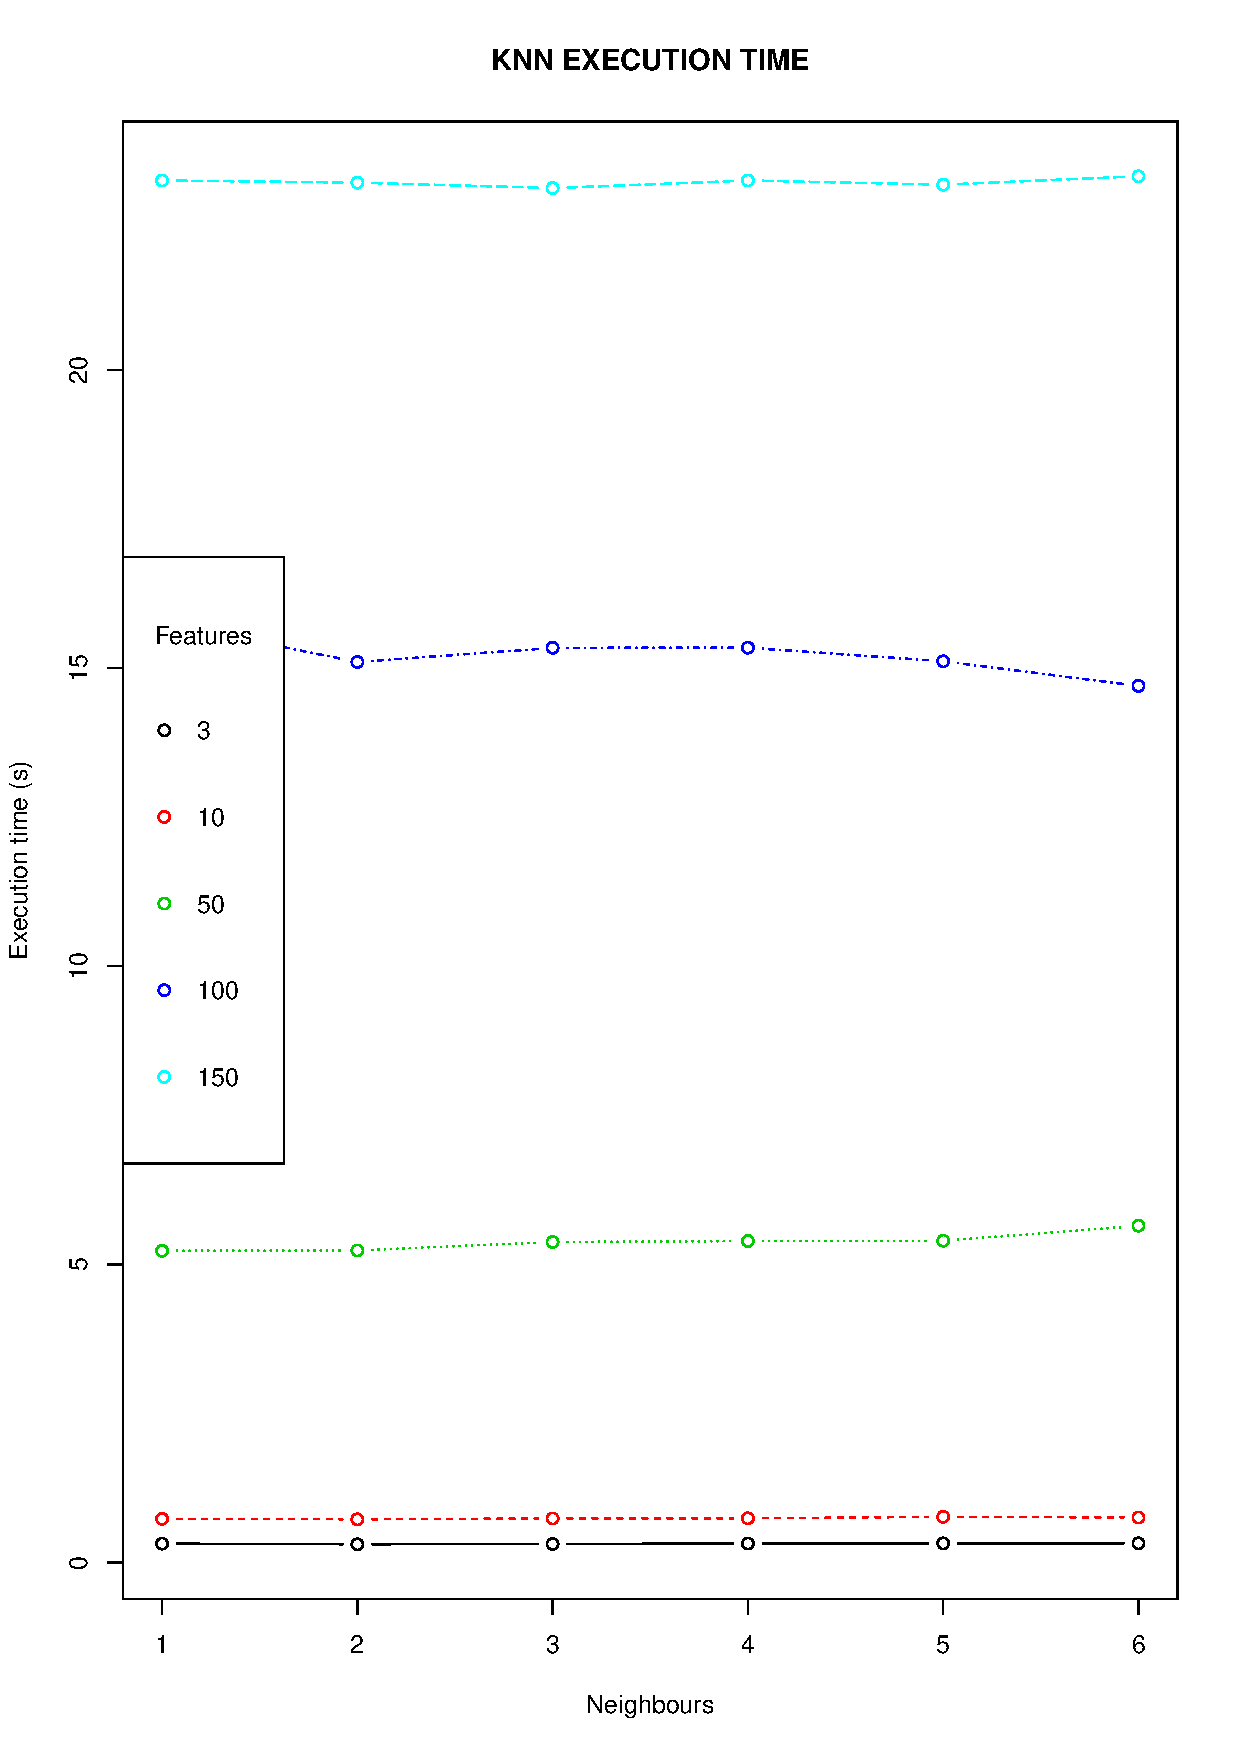
\includegraphics[scale=0.3]{../knn_time_rgb.pdf}  
     }
     \centering
     \caption{Execution time knn}
      \end{adjustwidth}
   \end{figure}
   
\noindent Overall, the baseline is very promising but hard to improve. The knn algorithm seems to be very suitable to classify images.

\subsection{Support Vector Machines}
Support vector machines (svm) are often used in image classification, in thier simplest form they are just linear classifiers. However the dataset seems to be hardly linearly separable, therefore the gaussian kernel was applied to allow generic curves to be used. The gaussian kernel is a linear combination of polynomial kernels that allows for more accurate predictions but slows down the algorithm.\\
The plot on the left of figure \ref{svmaccuracy} show the accuracy of the svm on the grayscale features. The svm reaches a lower accuracy with respect to the accuracy of the knn algorithm: it is less precise by 0.02/0.03. On the countrary, svm with rgb features performs as well as the knn algorithm.\\
In both cases the best accuracy, as before, is reached when the number of features is 50.

\begin{figure}[H]  
  \begin{adjustwidth}{-4cm}{-4cm}
     \subfloat{%
       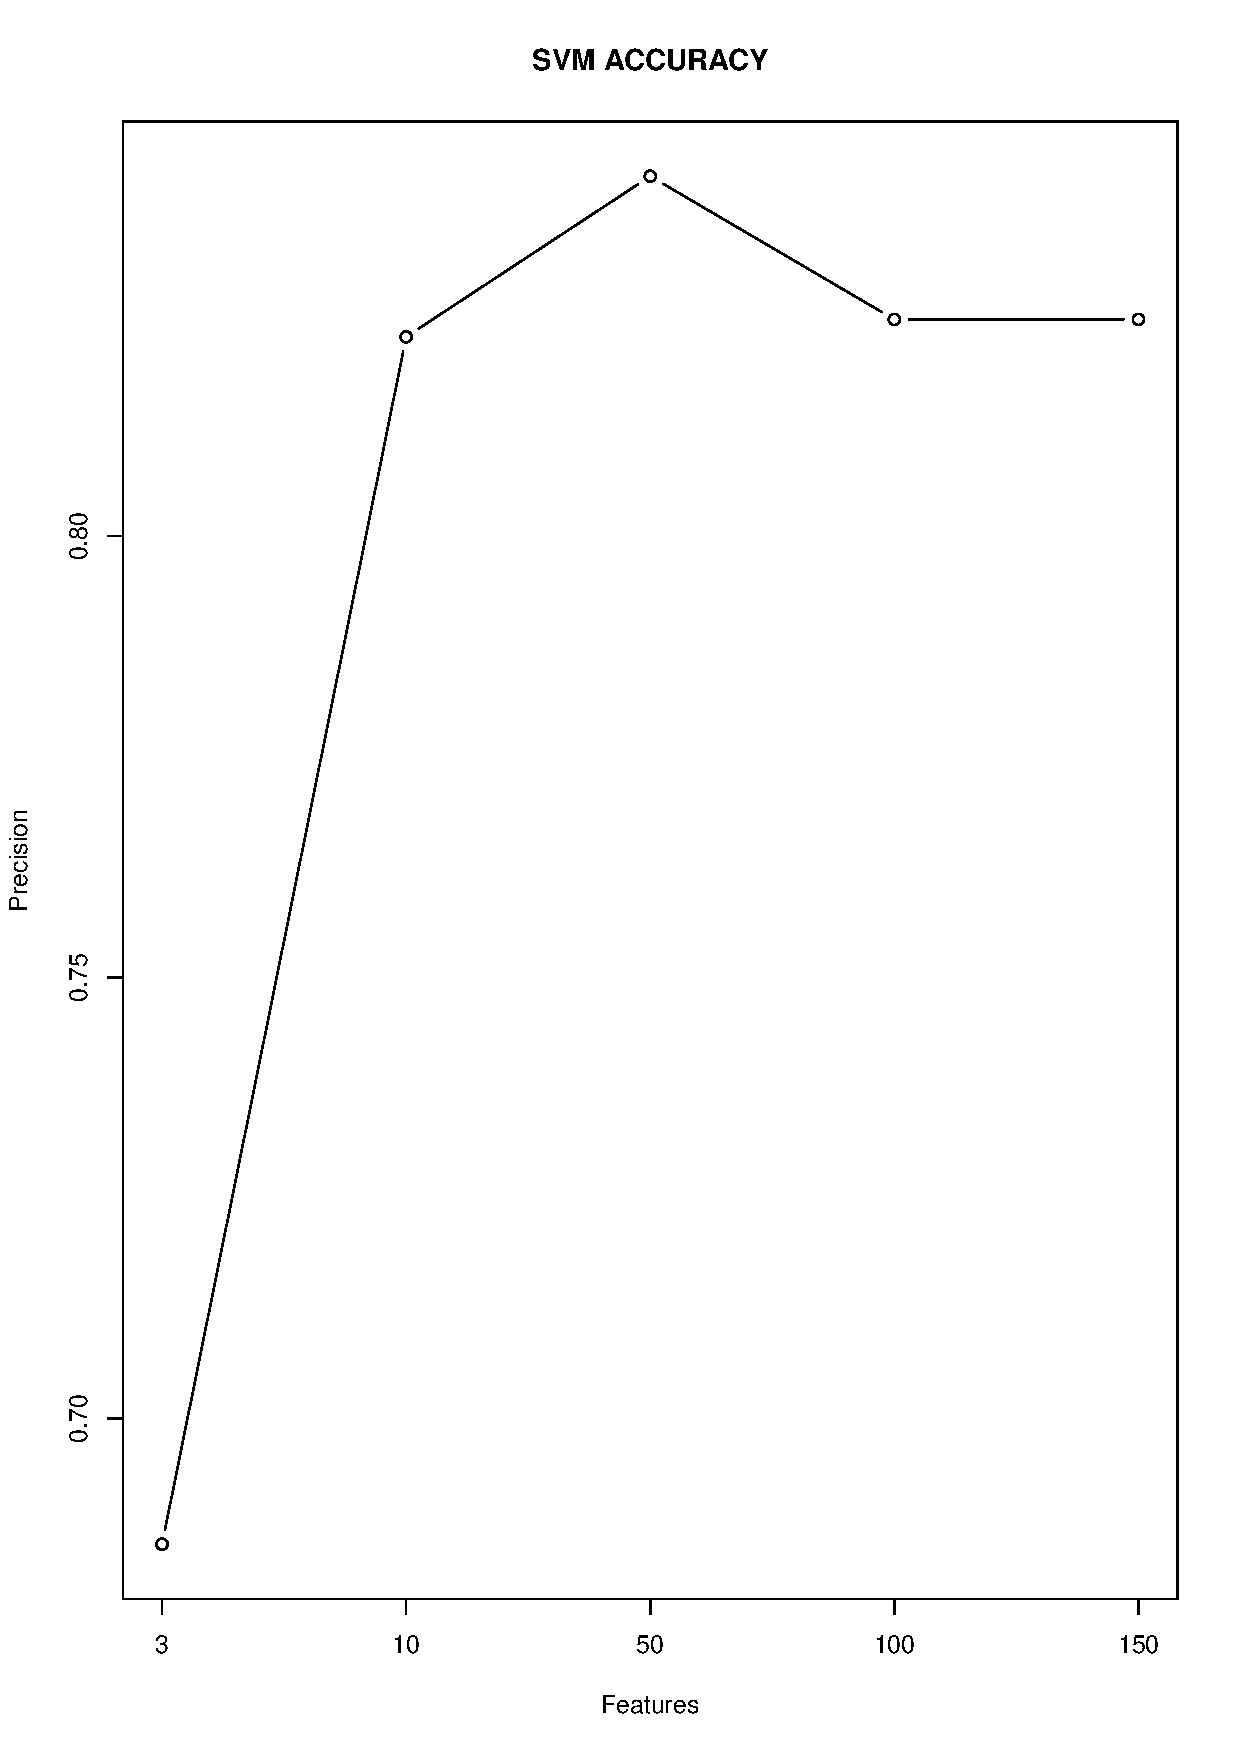
\includegraphics[scale=0.3]{../svm_accuracy_grayscale.pdf}
     }
     \subfloat{%
    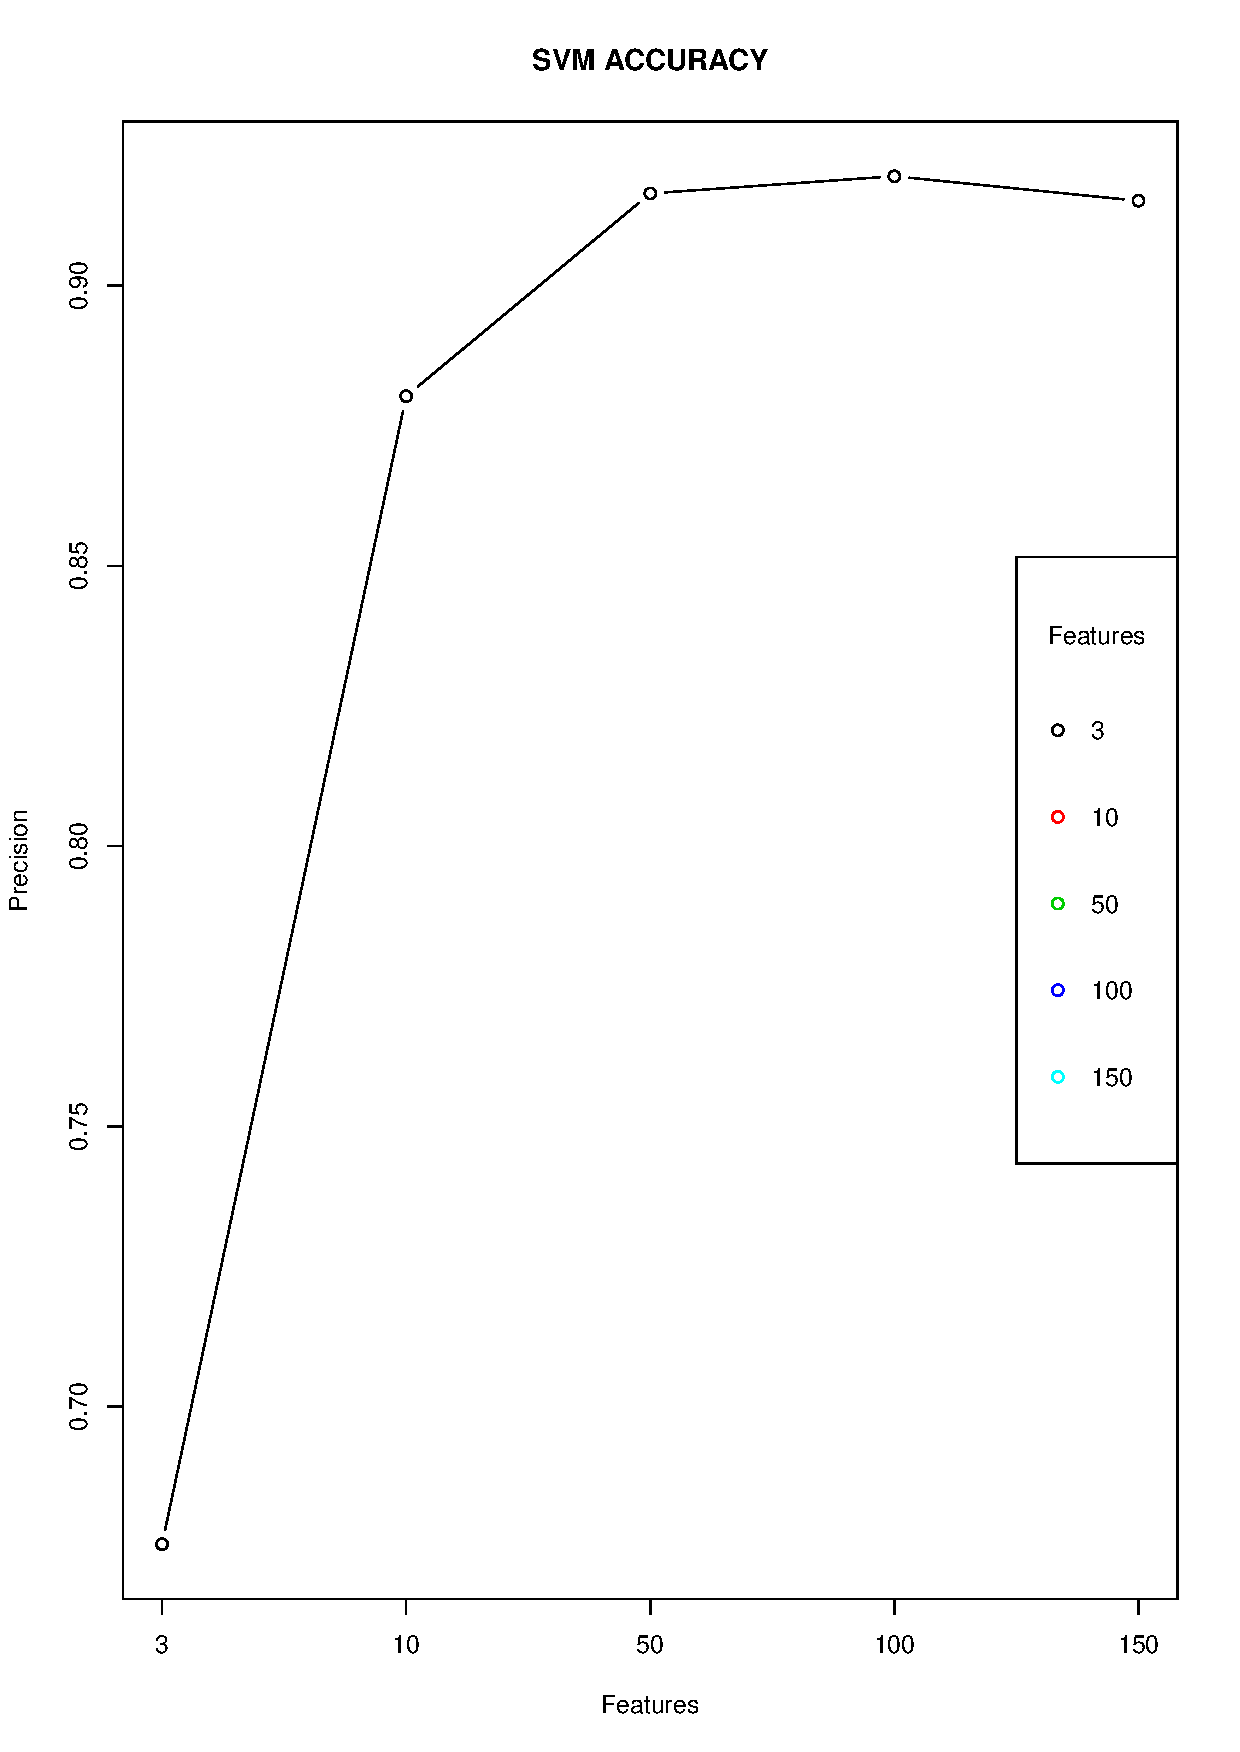
\includegraphics[scale=0.3]{../svm_accuracy_rgb.pdf}  
     }
     \centering
     \caption{Test accuracy svm} \label{svmaccuracy}
      \end{adjustwidth}
   \end{figure}

\noindent The execution time of the svm is way higher than the execution time of the knn, however it remains reasonable as figure \ref{svm time} shows.
   
\begin{figure}[H] 
  \begin{adjustwidth}{-4cm}{-4cm}
     \subfloat{%
       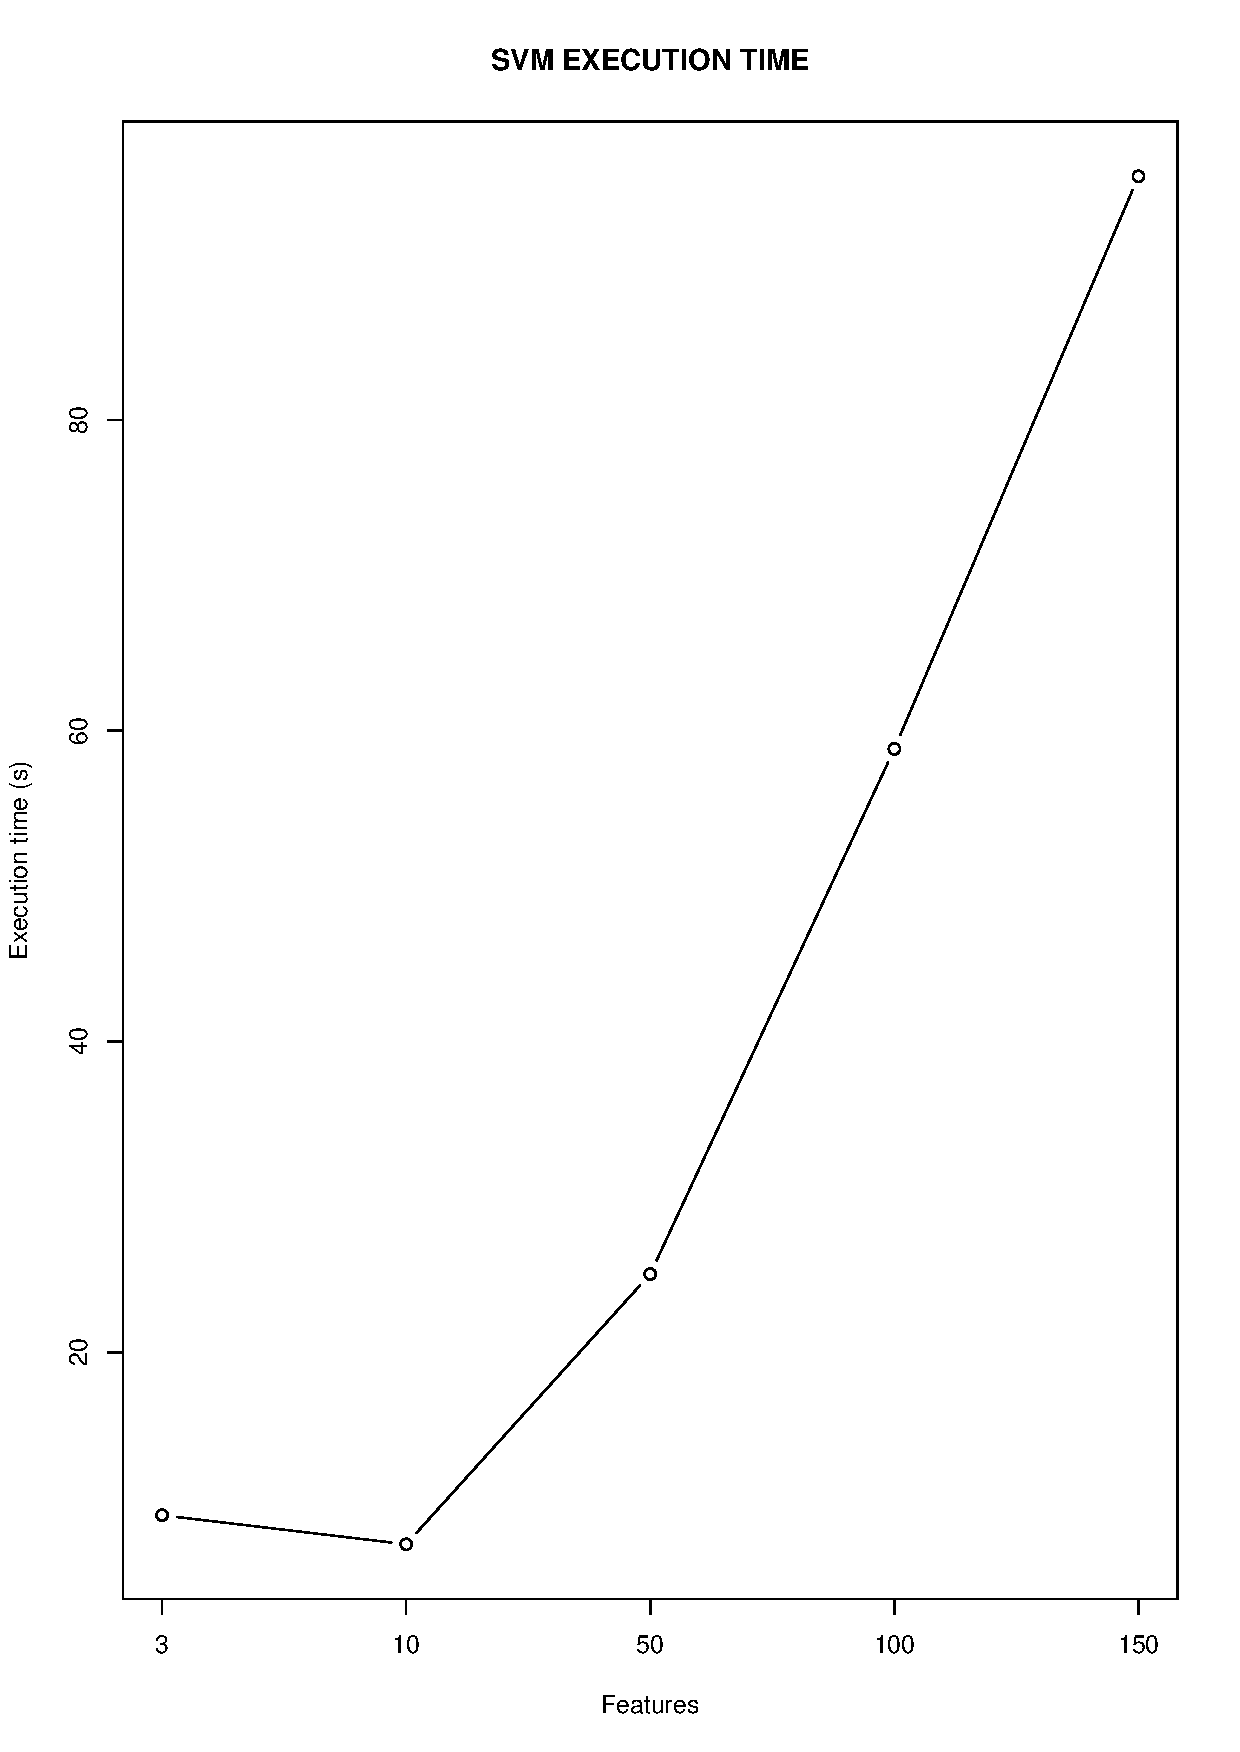
\includegraphics[scale=0.3]{../svm_time_grayscale.pdf}
     }
     \subfloat{%
    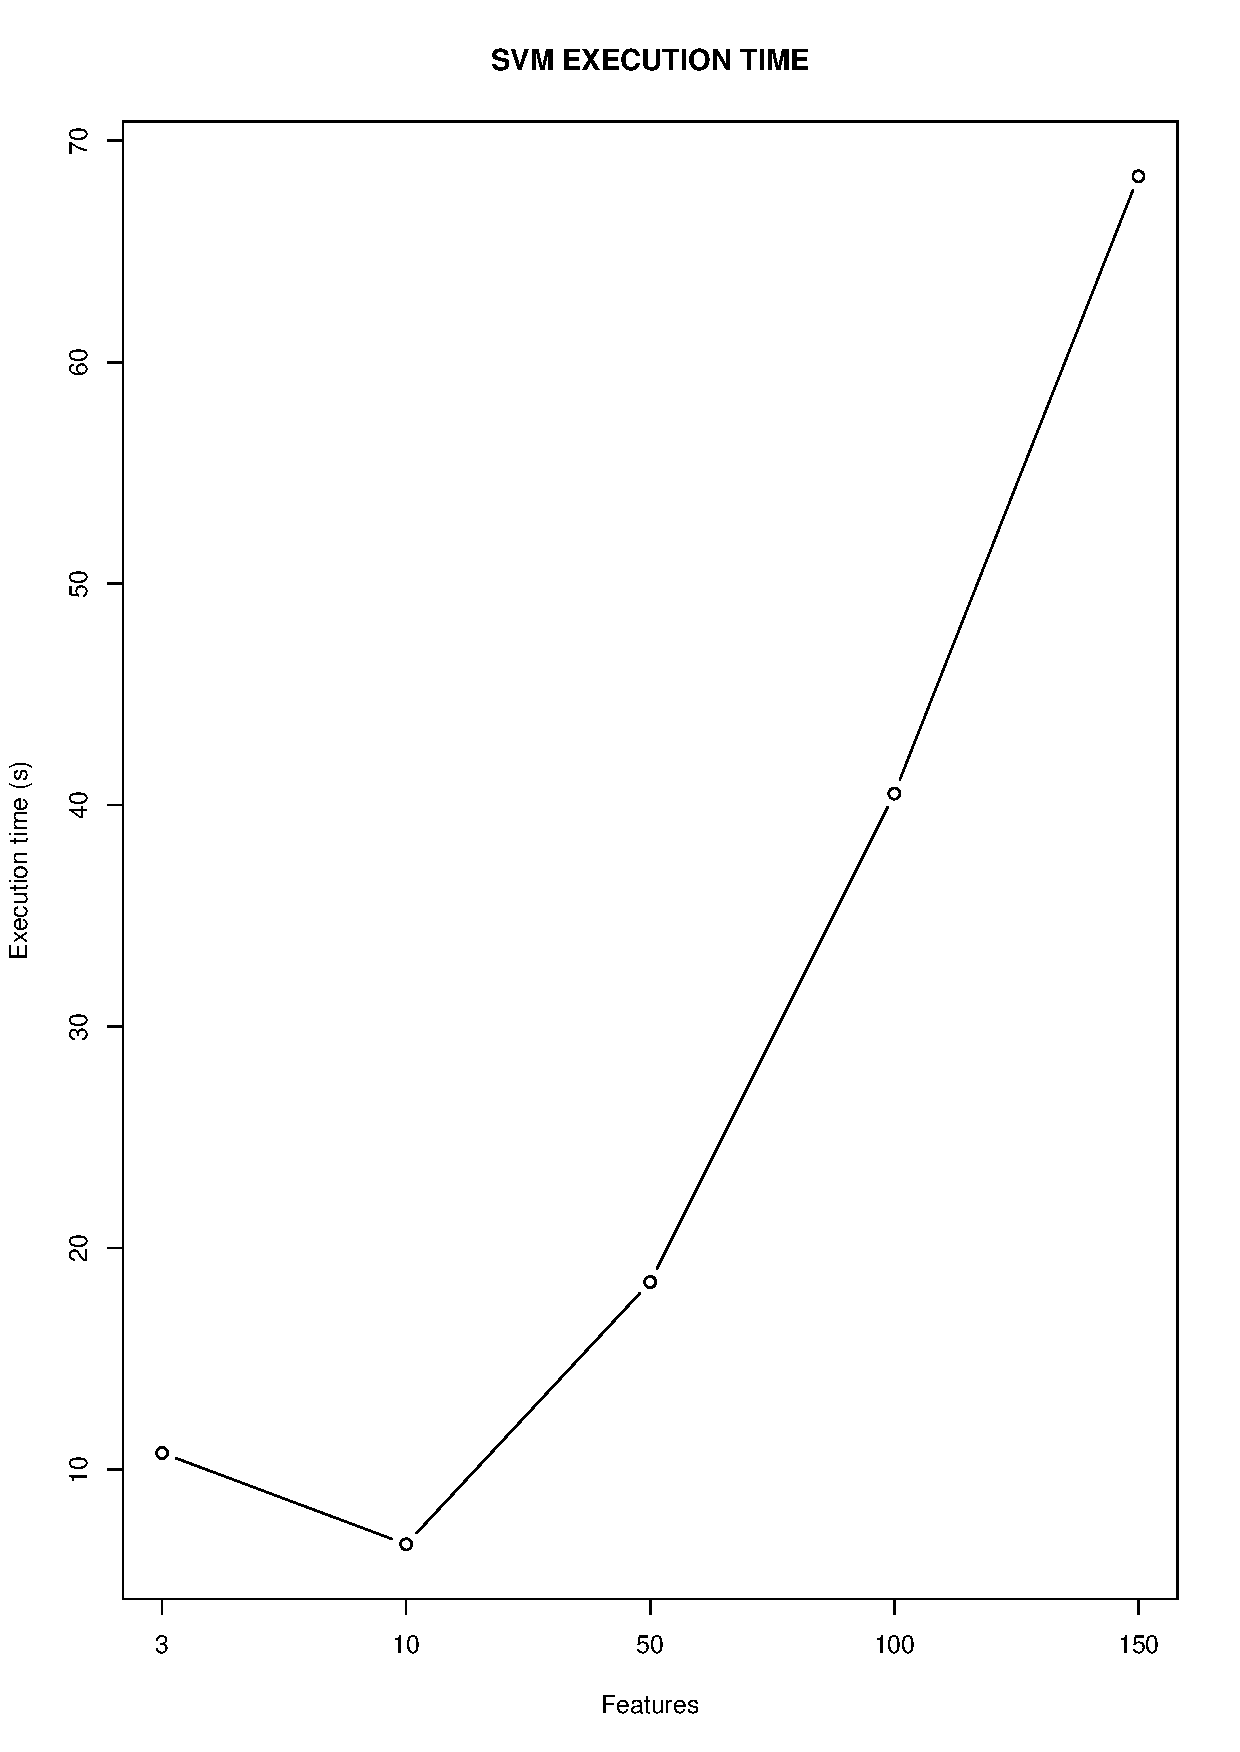
\includegraphics[scale=0.3]{../svm_time_rgb.pdf}  
     }
     \centering
     \caption{Execution time svm}  \label{svm time} 
      \end{adjustwidth}
   \end{figure}
\noindent Overall, the svm does not improve the result defined in the baseline that remains still very significant. Only a negliglible improvement is reached when using the rgb features. \\


\subsection{Convolutional neural network}
Deep learning algorithms are a class of machine learning algorithms often used to solve classification problems by exploiting multiple layers to extract higher level features. Among the various deep learning algorithms convolutional neural netwoks (CNN) are suitable for image classification since they can recognize translation invariant features. The topology of a  CNN consists in a stack of convolutional and pooling layers followed by dense layers. \\
Convolutional layers optimize the matrices known as filters that are applied to each portion of the data. It is worth noticing that the name convolutional neural network origins form the filtering operation known as discrete convolution in mathematics. \\ 
The pooling layer extracts a reduced representation of the data computed in the convolutional layer. Indeed, in this layer the dimensionality of the data is reduced by selecting a subset of the image and extracting a single value from each subset; usually the highest, mean or minimum value in the subset is extracted. \\
The process can be repeated by stacking convolutional and pooling layers; then, some fully connceted layers are stacked upon them. The purpose of these layers is to compute the probability that the input image belongs to each class. Therefore, the last layer of the net has a number of neurons equal to the number of class and the output is computed exploiting the \textit{softmax} function that provides a probability distribution. The prediction computed is the class having the hights probability. \\
The main reason to prefer deep learning techniques  to generic neural networks is that many layers with fewer weights are more flexible and precise in classification than neural networks with many weights and fewer layers. CNNs are also very computationally efficient because they optimize only the small filters in the convolutional layers and just few dense layers whose optimization is computationally more expensive. \\
The implementation of the CNNs relies on the \textit{Keras} and \textit{tensorflow} API.\\
Figure \ref{cnn} shows the training accuracy of the CNN with respect to the number of epochs in the training process. The training accuracy reachs as high as 0.99 while the test accuracy is a bit lower for both grayscale and rgb features.
When grayscale features are involved the test accuracy of the CNN is about 0.90, while is 0.94 when considering rgb features.
\begin{figure}[H] 
  \begin{adjustwidth}{-4cm}{-4cm}
     \subfloat{%
      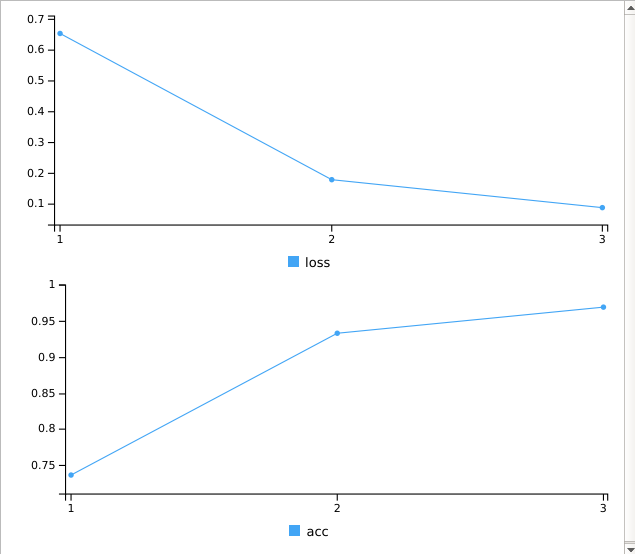
\includegraphics[scale=0.3]{../cnn_grayscale.png} 
     }
     \subfloat{%
 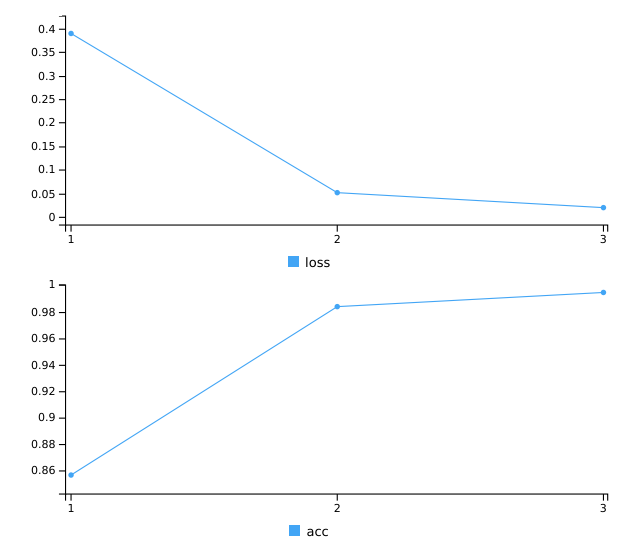
\includegraphics[scale=0.3]{../cnn_rgb.png} 
     }
     \centering
     \caption{CNN training accuracy} \label{cnn} 
      \end{adjustwidth}
   \end{figure}
\noindent The training time of both the nets is about 1 minute and the computation of the prediction requires about 30 seconds. Therefore CNN are faster than some instances of SVM but slower than the KNN.\\
Overall, the CNNs seem to be the best model to classify images.

\section{Conclusions}
This work aims to analyze the performance of well-known classification algorithms: k-nearest neighbour, support vector machines and convolutional neural networks on \textit{Fruit 360} dataset.\\
One of the most interesting result emerged from the analysis concenring KNN and SVM: theory suggests that SVM should have more predictive power and accuracy than KNN since it is far more complex. However, despite its simplicity KNN matches and even outperforms SVM. Moreover, this work confirms what other researches found out: CNN have the best performance and rgb features are very significant features even if they are easy to extract. To sustain the claim, the table \ref{results} was built: it presents the best accuracy for each algorithm and for each feature.
\begin{table}[H]
\centering
 \begin{tabular}{|c|c|c|c|} 
 \hline
  Algorithms & 1-NN & SVM & CNN\\
 \hline
 Grayscale&0.86&0.84&0.90 \\
 \hline
 Rgr&0.91& 0.92 & 0.94  \\
 \hline
\end{tabular}
\caption{Best accuracy scores} \label{results}
\end{table}
\noindent It is also worth noticing that the accuracy rate achieved using rgb features are higher than all the accuracy rate achieved with grayscale features. However, these results seem to be 4\% lower than the state-of-art in fruit classification. Indeed, the best accuracy rate reached in mixed fruit classification is 0.98 as reported in \cite{review}. However, the comparison is not straightforward since the dimension of the dataset and the number of classes is different. Moreover, most of the literature focuses on one vs all classification while this work handles multiclass classification. Nevertheless, the objective of the project were fulfilled:
\begin{enumerate}
\item Grayscale features allows to achieve the remarkable accuracy (0.90)
\item Rgb features provide an 0.04 improvement of the previous result
\item Despite its semplicity, Knn has a remarkable accuracy rate (0.91)
\end{enumerate}

\newpage
\section{Appendix: Code}
\begin{verbatim}
library(jpeg)
library(imager)
library(class)
library(e1071)
library(FactoMineR)
library(factoextra)
library(keras)
library(tensorflow)

read_fruit_grayscale <- function(path,set,fruit, dim = 50){
  filenames <- list.files(paste(path,set,fruit,sep=""), pattern = "*.jpg")
  images_grayscale = list()
  i = 1
  for (name in  filenames){
    path_name = paste(path,set,fruit,"/",name,sep="")
    img <- grayscale(load.image(path_name))
    inmg <- resize(img,dim,dim)
    images_grayscale[[i]] = as.vector(img)
    i = i+1
  }
  return(images_grayscale)
}


#number of pixels to be used
dim = 50
path = "../fruits-360_dataset/fruits-360/"

# grayscale extraction
set = "Training/"
training_features_matrix <- NULL
training_labels_vector <- NULL

fruits = c ("Apple Golden 1", "Apple Golden 2", 
"Apple Red 2","Apple Red 1", "Banana", "Apricot", "Blueberry")
i = 0
for (fruit in fruits){
  images_grayscale <- read_fruit_grayscale(path,set,fruit)
  images_grayscale <- matrix(unlist(images_grayscale), ncol = dim*dim, byrow = TRUE)
  training_features_matrix <- rbind(training_features_matrix,images_grayscale)
  labels <-replicate(dim(images_grayscale)[1], i)
  training_labels_vector <- c(training_labels_vector,labels)
  i <- i +1
}


set = "Test/"
test_features_matrix <- NULL
test_labels_vector <- NULL
i = 0
for (fruit in fruits){
  images_grayscale <- read_fruit_grayscale(path,set,fruit)
  images_grayscale <- matrix(unlist(images_grayscale), ncol = dim*dim, byrow = TRUE)
  test_features_matrix <- rbind(test_features_matrix,images_grayscale)
  labels <-replicate(dim(images_grayscale)[1], i)
  test_labels_vector <- c(test_labels_vector,labels)
  i <- i +1
}


#PCA
t1 <- Sys.time()
pca <- prcomp(training_features_matrix,center = TRUE, scale=TRUE)
t2 <- Sys.time()
pca_execution_time <- t2 - t1
# pca_execution_time = Time difference of 5.653888 mins
pr_var <- (pca$sdev[1:200])^2
prop_varex <- pr_var/sum(pr_var)
plot(cumsum(prop_varex), xlab = "Principal Component",
     ylab = "Cumulative Proportion of Variance Explained")


training_features_matrix_pc <- pca$x
test_features_matrix_pc <- predict(pca, newdata = test_features_matrix)

#BASELINE
neighbours <- c(1,3,5,7,9,11)
features <- c(3,10,50,100,150)
res_knn <- c()
time_knn <- c()
i <- 1
for (n_f in features){
  for (n in neighbours){
    t1 <- Sys.time()
    knn <-knn(training_features_matrix_pc[,1:n_f], test_features_matrix_pc[,1:n_f], 
      as.factor(training_labels_vector), k=n)
    t2 <- Sys.time()
    time_knn[i] <- as.double(difftime(t2,t1,  units = "secs"))
    res_knn[i] <- sum(knn == test_labels_vector)/length(test_labels_vector)
    i <- i +1
  }
}

time_knn

res_knn 

precision <- matrix(res_knn,ncol=length(features))
matplot(precision, type = c("b"),pch=1,  xlab = "Neighbours",
 ylab="Accuracy", main="KNN ACCUARCY", xaxt = "n")
axis(1, at=1:length(neighbours), labels=neighbours)
legend("left", legend = features, col=1:length(features), pch=1, title="Features")

time <- matrix(time_knn,ncol=length(features))
matplot(time, type = c("b"),pch=1, xaxt = "n", xlab = "Neighbours", 
ylab="Execution time (s)", main="KNN EXECUTION TIME")
axis(1, at=1:length(neighbours), labels=neighbours)
legend("right", legend = features, col=1:length(features), pch=0.5, title="Features" ,cex = 0.7)

features <- c(3,10,50,100,150)
res_svm <- c()
time_svm <- c()
i <- 1
for (n_f in features){
  training_features_matrix_svm <- as.data.frame(training_features_matrix_pc[,1:n_f])
  training_features_matrix_svm$target <- as.factor(training_labels_vector)
  test_features_matrix_svm <- as.data.frame(test_features_matrix_pc[,1:n_f])
  
  t1 <- Sys.time()
  SVM <- svm(target ~ ., data = training_features_matrix_svm, kernel = "radial")
  t2 <- Sys.time()
  res <- predict(SVM, newdata = test_features_matrix_svm)
  time_svm[i] <- as.double(difftime(t2,t1,  units = "secs"))
  res_svm[i] <-     sum(res == test_labels_vector)/length(test_labels_vector)
  i <- i +1
}

time_svm
res_svm 

plot(res_svm, type = c("b"),pch=1 , xlab = "Features", 
ylab="Precision", main="SVM ACCURACY", xaxt = "n")
axis(1, at=1:length(features), labels=features)


plot(time_svm, type = c("b"),pch=1 , xlab = "Features", 
ylab="Execution time (s)", main="SVM EXECUTION TIME", xaxt = "n")
axis(1, at=1:length(features), labels=features)


#CNN KERAS

y_train <- to_categorical(training_labels_vector, length(fruits))
y_test <- to_categorical(test_labels_vector, length(fruits))
x_train<-array_reshape(training_features_matrix,c(nrow(training_features_matrix),dim,dim,1))
x_test<-array_reshape(test_features_matrix,c(nrow(test_features_matrix),dim,dim,1))

model <- keras_model_sequential() %>%
  layer_conv_2d(filters = 16, kernel_size = c(3, 3), activation = "relu",
                input_shape = c(50, 50, 1)) %>%
  layer_max_pooling_2d(pool_size = c(4,4)) %>%
  layer_conv_2d(filters = 64, kernel_size = c(2, 2), activation = "relu") %>%
  layer_flatten() %>%
  layer_dropout(rate=0.5) %>%
  layer_dense(units = 300, activation = "relu") %>%
  layer_dense(units = 200, activation = "tanh") %>%
  layer_dense(units = length(fruits), activation = "softmax")

model <- keras_model_sequential() %>%
  layer_conv_2d(filters = 16, kernel_size = c(3, 3), activation = "relu",
                input_shape = c(50, 50, 1)) %>%
  layer_max_pooling_2d(pool_size = c(4,4)) %>%
  layer_conv_2d(filters = 32, kernel_size = c(3, 3), activation = "relu") %>%
  layer_max_pooling_2d(pool_size = c(4, 4)) %>%
  #layer_conv_2d(filters = 128, kernel_size = c(2, 2), activation = "tanh") %>%
  #layer_max_pooling_2d(pool_size = c(4, 4)) %>%
  #layer_conv_2d(filters = 128, kernel_size = c(2, 2), activation = "tanh") %>%
  layer_flatten() %>%
  layer_dropout(rate=0.4) %>%
  layer_dense(units = 300, activation = "relu") %>%
  layer_dense(units = 200, activation = "relu") %>%
  layer_dense(units = length(fruits), activation = "softmax")

model %>% compile(
  optimizer='adam',
  loss='categorical_crossentropy',
  metrics='accuracy')

t1 <- Sys.time()
history<- model %>% fit(
  x_train,y_train,
  epochs=3,
  batch_size=50)
t2 <- Sys.time()
cnn_execution_time <-  as.double(difftime(t2,t1,  units = "secs"))
model %>% evaluate(x_test, y_test)

#RGB ANALYSIS
read_fruit_rgb <- function(path,set,fruit, dim = 50){
  filenames <- list.files(paste(path,set,fruit,sep=""), pattern = "*.jpg")
  images_rgb= list()
  i = 1
  for (name in  filenames){
    path_name = paste(path,set,fruit,"/",name,sep="")
    img <- load.image(path_name)
    inmg <- resize(img,dim,dim)
    images_rgb[[i]] = as.vector(img)
    i = i+1
  }
  return(images_rgb)
}

#number of pixels to be used
dim = 50
path = "../fruits-360_dataset/fruits-360/"

# rgb extraction

set = "Training/"
training_labels_vector <- NULL
fruits = c ("Apple Golden 1", "Apple Golden 2", "Apple Red 2",
"Apple Red 1", "Banana", "Apricot", "Blueberry")

i = 0
training_features_matrix_rgb <- NULL
for (fruit in fruits){
  images_rgb <- read_fruit_rgb(path,set,fruit)
  images_rgb <- matrix(unlist(images_rgb), ncol = dim*dim*3, byrow = TRUE)
  labels <-replicate(dim(images_rgb)[1], i)
  training_labels_vector <- c(training_labels_vector,labels)
  training_features_matrix_rgb <- rbind(training_features_matrix_rgb,images_rgb)
  i <- i +1
}


set = "Test/"
test_labels_vector <- NULL

i = 0
test_features_matrix_rgb <- NULL
for (fruit in fruits){
  images_rgb <- read_fruit_rgb(path,set,fruit)
  images_rgb <- matrix(unlist(images_rgb), ncol = dim*dim*3, byrow = TRUE)
  test_features_matrix_rgb <- rbind(test_features_matrix_rgb,images_rgb)
  labels <-replicate(dim(images_rgb)[1], i)
  test_labels_vector <- c(test_labels_vector,labels)
  i <- i +1
}

#PCA
t1 <- Sys.time()
pca_rgb <- prcomp(training_features_matrix_rgb,center = TRUE, scale=TRUE)
t2 <- Sys.time()
pca_rgb_execution_time <- as.double(difftime(t2,t1,  units = "min")) # 57.14827 minutes
pr_var_rgb <- (pca_rgb$sdev[1:200])^2
prop_varex_rgb <- pr_var_rgb/sum(pr_var_rgb)
plot(cumsum(prop_varex_rgb), xlab = "Principal Component",
     ylab = "Cumulative Proportion of Variance Explained")

training_features_matrix_rgb_pc <- pca_rgb$x
test_features_matrix_rgb_pc <- predict(pca_rgb, newdata = test_features_matrix_rgb)

#KNN
neighbours <- c(1,3,5,7,9,11)
features <- c(3,10,50,100,150)
res_knn <- c()
time_knn <- c()
i <- 1
for (n_f in features){
  for (n in neighbours){
    t1 <- Sys.time()
    knn <-knn(training_features_matrix_rgb_pc[,1:n_f], test_features_matrix_rgb_pc[,1:n_f], as.factor(training_labels_vector), k=n)
    t2 <- Sys.time()
    time_knn[i] <- as.double(difftime(t2,t1,  units = "secs"))
    res_knn[i] <- sum(knn == test_labels_vector)/length(test_labels_vector)
    i <- i +1
  }
}

time_knn 
res_knn


precision <- matrix(res_knn,ncol=length(features))
matplot(precision, type = c("b"),pch=1,  xlab = "Neighbours", 
ylab="Accuracy", main="KNN ACCUARCY", xaxt = "n")
axis(1, at=1:length(neighbours), labels=neighbours)
legend("left", legend = features, col=1:length(features), pch=1, title="Features")

time <- matrix(time_knn,ncol=length(features))
matplot(time, type = c("b"),pch=1, xaxt = "n", xlab = "Neighbours", 
ylab="Execution time (s)", main="KNN EXECUTION TIME")
axis(1, at=1:length(neighbours), labels=neighbours)
legend("right", legend = features, col=1:length(features), pch=0.5, title="Features" ,cex = 0.65)

features <- c(3,10,50,100,150)
res_svm <- c()
time_svm <- c()
i <- 1
for (n_f in features){
  training_features_matrix_svm <- as.data.frame(training_features_matrix_rgb_pc[,1:n_f])
  training_features_matrix_svm$target <- as.factor(training_labels_vector)
  test_features_matrix_svm <- as.data.frame(test_features_matrix_rgb_pc[,1:n_f])
  
  t1 <- Sys.time()
  SVM <- svm(target ~ ., data = training_features_matrix_svm, kernel = "radial")
  t2 <- Sys.time()
  res <- predict(SVM, newdata = test_features_matrix_svm)
  time_svm[i] <- as.double(difftime(t2,t1,  units = "secs"))
  res_svm[i] <-     sum(res == test_labels_vector)/length(test_labels_vector)
  i <- i +1
}

time_svm
res_svm


plot(res_svm, type = c("b"),pch=1 , xlab = "Features", 
ylab="Precision", main="SVM ACCURACY", xaxt = "n")
axis(1, at=1:length(features), labels=features)
legend("right", legend = features, col=1:length(features), pch=1, title="Features")

plot(time_svm, type = c("b"),pch=1 , xlab = "Features", 
ylab="Execution time (s)", main="SVM EXECUTION TIME", xaxt = "n")
axis(1, at=1:length(features), labels=features)

features <- c(3,10,50,100,150)
res_svm <- c()
time_svm <- c()
i <- 1
for (n_f in features){
  training_features_matrix_svm <- as.data.frame(training_features_matrix_rgb_pc[,1:n_f])
  training_features_matrix_svm$target <- as.factor(training_labels_vector)
  test_features_matrix_svm <- as.data.frame(test_features_matrix_rgb_pc[,1:n_f])
  
  t1 <- Sys.time()
  SVM <- svm(target ~ ., data = training_features_matrix_svm, kernel = "radial")
  t2 <- Sys.time()
  res <- predict(SVM, newdata = test_features_matrix_svm)
  time_svm[i] <- as.double(difftime(t2,t1,  units = "secs"))
  res_svm[i] <-     sum(res == test_labels_vector)/length(test_labels_vector)
  i <- i +1
}

time_svm
#[1] 11.048466  7.334074 20.145182 42.065335 66.613935 radial kernel
res_svm 
#0.6754386 0.8802632 0.9164474 0.9195175 0.9151316 radial kernel

plot(res_svm, type = c("b"),pch=1 , xlab = "Features", ylab="Precision", main="SVM ACCURACY", xaxt = "n")
axis(1, at=1:length(features), labels=features)

plot(time_svm, type = c("b"),pch=1 , xlab = "Features", ylab="Execution time (s)", main="SVM EXECUTION TIME", xaxt = "n")
axis(1, at=1:length(features), labels=features)



y_train <- to_categorical(training_labels_vector, length(fruits))
y_test <- to_categorical(test_labels_vector, length(fruits))
x_train<-array(training_features_matrix_rgb,c(nrow(training_features_matrix_rgb),dim,dim,3))
x_test<-array(test_features_matrix_rgb,c(nrow(test_features_matrix_rgb),dim,dim,3))

model <- keras_model_sequential() %>%
  layer_conv_2d(filters = 16, kernel_size = c(3, 3), activation = "relu",
                input_shape = c(50, 50, 3)) %>%
  layer_max_pooling_2d(pool_size = c(4,4)) %>%
  layer_conv_2d(filters = 64, kernel_size = c(2, 2), activation = "relu") %>%
  layer_flatten() %>%
  layer_dropout(rate=0.5) %>%
  layer_dense(units = 300, activation = "relu") %>%
  layer_dense(units = 200, activation = "tanh") %>%
  layer_dense(units = length(fruits), activation = "softmax")

model %>% compile(
  optimizer='adam',
  loss='categorical_crossentropy',
  metrics='accuracy')

t1 <- Sys.time()
history<- model %>% fit(
  x_train,y_train,
  epochs=3,
  batch_size=50)
t2 <- Sys.time()
cnn_execution_time <-  as.double(difftime(t2,t1,  units = "secs"))
model %>% evaluate(x_test, y_test)

\end{verbatim}

\newpage
\begin{thebibliography}{9}

\bibitem{dataset}
\textit{Horea Muresan, Mihai Oltean, Fruit recognition from images using deep learning, Acta Univ. Sapientiae, Informatica Vol. 10, Issue 1, pp. 26-42, 2018.}

\bibitem{review}
\textit{Khurram Hameed, Douglas Chai, Alexander Rassau, A comprehensive review of fruit and vegetable classification techniques. Image and Vision Computing 80 (2018) 22-44.} 

\bibitem{grayscaleconversion}
\textit{Samuel Macedo, Givanio Melo, Judith Kelner, A comparative study of grayscale conversion techniques applied to SIFT descriptors, SBC Journal on Interactive Systems, volume 6, number 2, 2015.}

\bibitem{knnresults}
\textit{Sandeep Kumar, Zeeshan Khan, Anurag jain, A Review of Content Based Image Classification using Machine Learning Approach, International Journal of Advanced Computer Research (ISSN (print): 2249-7277 ISSN (online): 2277-7970) Volume-2 Number-3 Issue-5 September-2012}

\end{thebibliography} 
\end{document}


